\chapter{TP Monitors}

	\section{Terminology}
		1. All steps necessery to perform some kind of business transaction\\
		OR\\
		2. The execution of a programm that implements a business transaction
		
	\section{Purpose of TPM's}
		An application is written to perform a SINGLE request, the TP Monitor is responsible for scaling this application up, so that many transactions can be done at the same Time.
		
	
	\section{Transaction Application Structure}
	
		\begin{figure}[h!]
			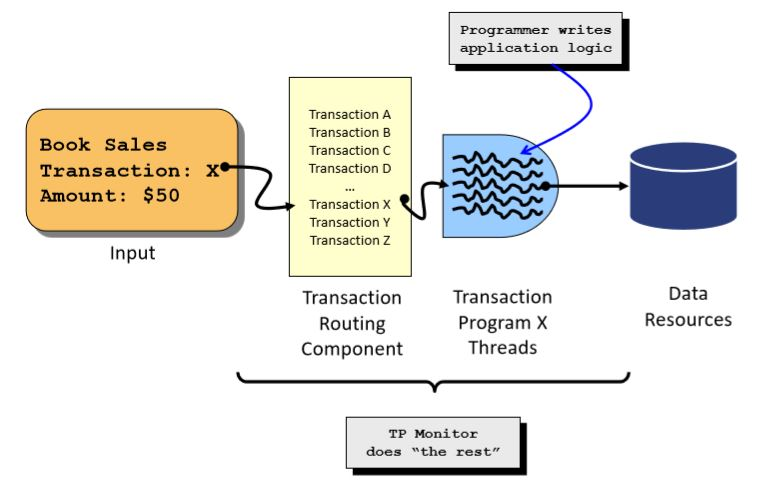
\includegraphics[scale=0.5]{res/transaction_application_structure.jpg}
			\caption{Transaction Application Structure}
		\end{figure}
	
	\section{TPM Structure}
		\begin{itemize}
			\item Presentation server
				\subitem gathers the input
				\subitem helps configuring the transaction request
				\subitem initial validation and authentication 
			\item Control flow server
				\subitem Request routing
				\subitem Transaction bracketing
				\subitem Request message integrity
				\subitem Exception handling
			\item Transaction server
				\subitem Logic execution
				\subitem resource manipulation
		\end{itemize}
	
	\section{Security}
		\begin{itemize}
			\item Presentation server authenticates 
				\subitem the location (users device)
				\subitem the user
			\item Control flow server authenticates
				\subitem the presentation server
				\subitem the location (users device)
				\subitem the user
		\end{itemize}
		\begin{figure}[h!]
			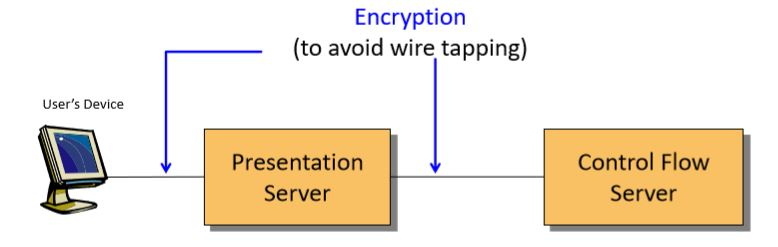
\includegraphics[scale=0.5]{res/tpm_security.jpg}
			\caption{TPM Security}
		\end{figure}
	
		
	\section{Presentation server request structure}
		The presentation server gathers the input and structures the information as follows:
			